\documentclass[12pt,a4paper]{ctexart}
\usepackage[margin=2.2cm]{geometry}
\usepackage{graphicx}
\usepackage{booktabs}
\usepackage{amsmath}
\usepackage{amssymb}
\usepackage{float}
\usepackage{hyperref}
\usepackage{xcolor}
\usepackage{listings}
\usepackage{subcaption}

\lstset{
  language=Python,
  basicstyle=\ttfamily\small,
  keywordstyle=\color{blue!70!black},
  commentstyle=\color{green!40!black},
  stringstyle=\color{orange!60!black},
  showstringspaces=false,
  breaklines=true,
  frame=single,
  tabsize=4
}

\newcommand{\reporttitle}{Project 3：线性回归与线性分类实验报告}
\newcommand{\authname}{姓名}
\newcommand{\authid}{学号}
\newcommand{\class}{班级}

\title{\reporttitle}
\author{\authname：\underline{李祥熙} \quad \authid：\underline{2234412799} \quad \class：\underline{计算机2301}}
\date{}

\begin{document}
\maketitle
\tableofcontents
\newpage

% =====================================================================
\section{实验目的}
% =====================================================================

本实验的目标如下：

\begin{itemize}
  \item \textbf{掌握线性回归的三种求解方法}：分别从数学推导和代码实现的角度，深入理解解析解（闭式解）、全批量梯度下降（GD）和随机梯度下降（SGD）三种方式在参数优化中的原理与差异，并在年龄估计任务上对三种方法进行对比评估。
  \item \textbf{掌握线性感知机的实现与训练}：理解感知机模型的结构（权重向量 $\mathbf{w}$ 与偏置 $b$）、前向预测（\texttt{predict}）与反向更新（\texttt{update}）过程，基于梯度下降法实现 Primal Perceptron，并在 Emoji 二分类数据集上验证其收敛性。
  \item \textbf{理解辅助模块的设计}：由于实验提供的 \texttt{helperP.pyc} 编译自 Python 3.8，与当前 Python 3.14 环境不兼容，需要根据两份实验代码（Notebook）中的调用接口，完整重建 \texttt{helperP.py}，包括数据加载、性能评估、结果保存和可视化等功能。
\end{itemize}

% =====================================================================
\section{实验过程}
% =====================================================================

\subsection{实验环境}

\begin{itemize}
  \item 操作系统：Linux（Arch Linux，内核 7.0.11-arch1-1）
  \item 编程语言：Python 3.14.5
  \item 主要工具：NumPy 2.4.6、Matplotlib 3.10.9、Pillow 12.2.0、Jupyter Notebook
\end{itemize}

\subsection{数据集描述}

本实验使用两份数据集，分别对应线性回归和线性分类两个子任务。

\subsubsection{年龄估计数据集（线性回归）}

年龄估计数据集包含人脸图像，目标是从图像特征中预测人物年龄。预训练神经网络已将图像转换为 2048 维特征向量，存储在 \texttt{.npy} 文件中，标签（年龄）存储于对应的 \texttt{.txt} 文件中。数据集按如下方式划分：

\begin{itemize}
  \item \textbf{训练集}：3995 个样本，特征矩阵 $X_\text{train} \in \mathbb{R}^{3995 \times 2048}$，年龄向量 $\mathbf{y}_\text{train} \in \mathbb{R}^{3995}$
  \item \textbf{验证集}：1500 个样本，特征矩阵 $X_\text{val} \in \mathbb{R}^{1500 \times 2048}$，年龄向量 $\mathbf{y}_\text{val} \in \mathbb{R}^{1500}$
  \item \textbf{测试集}：500 个样本，特征矩阵 $X_\text{test} \in \mathbb{R}^{500 \times 2048}$，标签不提供
\end{itemize}

特征统计：均值 $\approx 0.170$，标准差 $\approx 0.242$，最大值 $\approx 10.87$，最小值为 0（ReLU 激活后的输出）。年龄范围约为 $[1, 90]$ 岁，均值约为 30.3 岁，标准差约为 14.7 岁。图~\ref{fig:age_dataset} 展示了验证集中的若干样本图像及其对应年龄。

\begin{figure}[H]
\centering
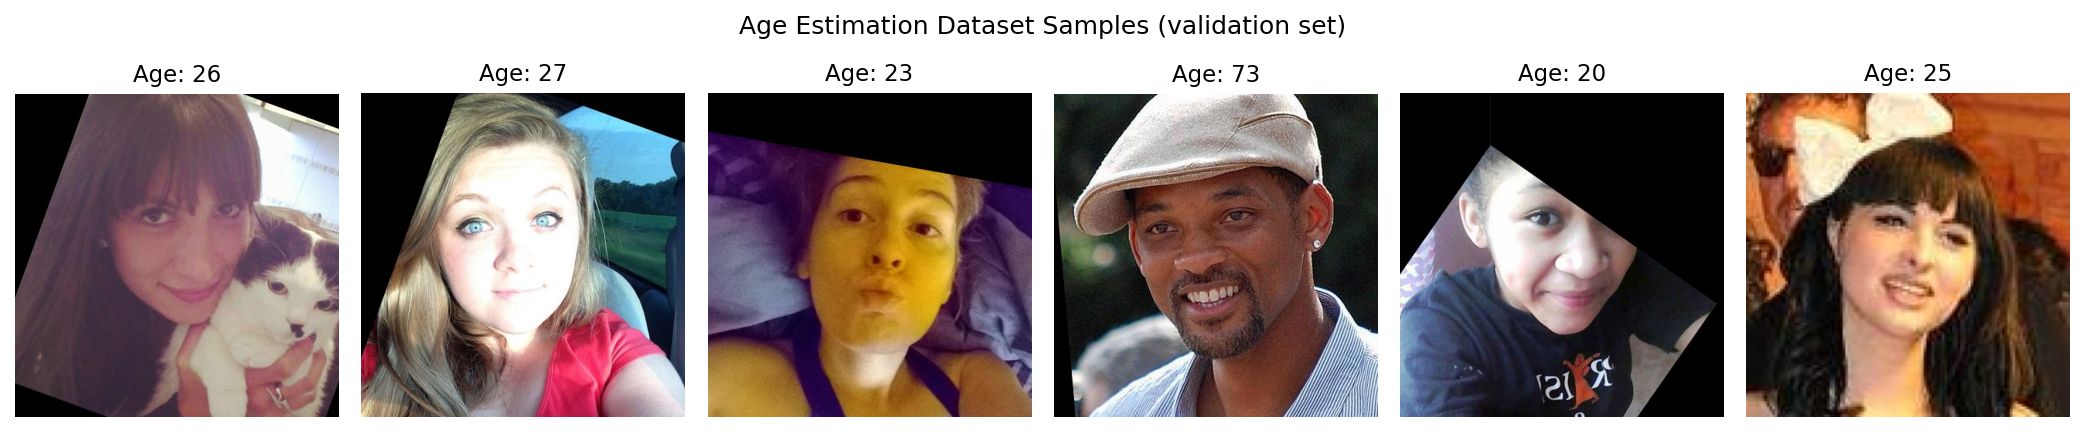
\includegraphics[width=0.98\textwidth]{images/age_dataset.png}
\caption{年龄估计数据集样本（验证集前 6 张图像及其真实年龄）}
\label{fig:age_dataset}
\end{figure}

\subsubsection{Emoji 数据集（线性分类）}

Emoji 数据集由 20 张 $160 \times 160$ 像素的 Emoji 图像组成，分为两类：
\begin{itemize}
  \item \texttt{train\_nosmile}：10 张不笑脸 Emoji，标签为 $-1$
  \item \texttt{train\_smile}：10 张笑脸 Emoji，标签为 $+1$
\end{itemize}

图像加载时转换为 $32 \times 32$ 灰度图并归一化至 $[0, 1]$，展开后得到 1024 维特征向量。图~\ref{fig:emoji_dataset} 展示了完整的 20 张 Emoji 及其真实标签（红色为 $-1$，蓝色为 $+1$）。

\begin{figure}[H]
\centering
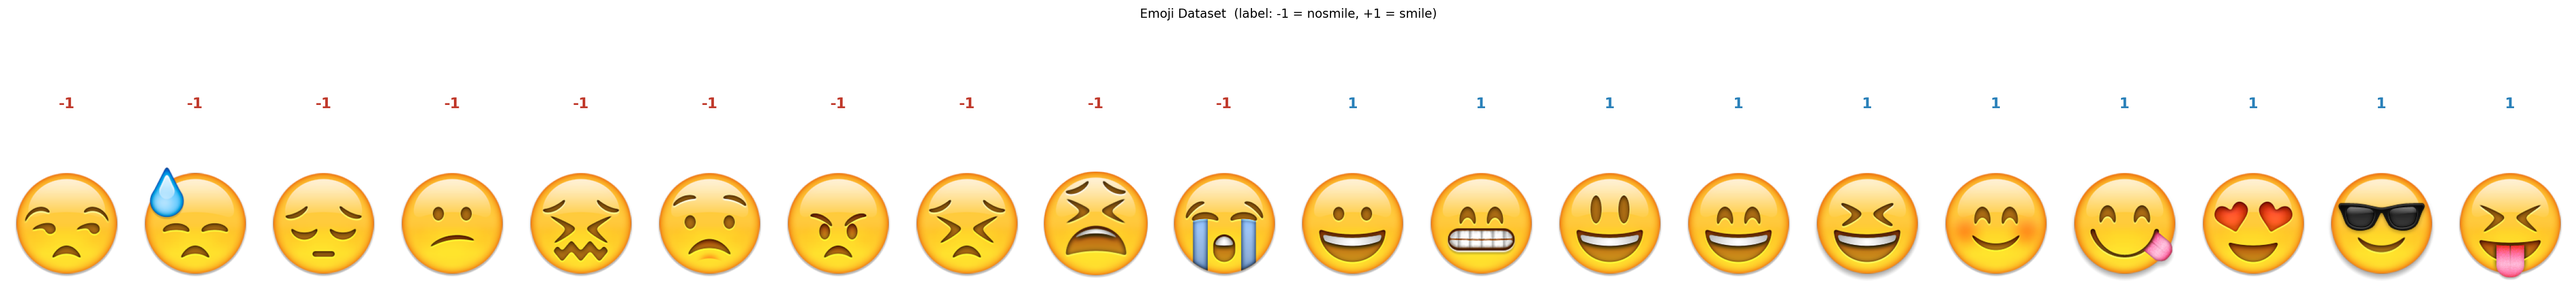
\includegraphics[width=0.98\textwidth]{images/emoji_dataset.png}
\caption{Emoji 数据集（上方数字为真实标签：$-1$ = 不笑脸，$+1$ = 笑脸）}
\label{fig:emoji_dataset}
\end{figure}

\subsection{辅助模块重建}

由于 \texttt{helperP.pyc} 由 Python 3.8 编译，Python 3.14 无法读取（\texttt{bad magic number} 错误），需要根据两份 Notebook 中的调用接口手动重建 \texttt{helperP.py}。重建的接口如下：

\begin{itemize}
  \item \texttt{prepare\_data(split, base\_dir)}：加载指定分割（train/val/test）的特征 \texttt{.npy} 文件和年龄 \texttt{.txt} 文件
  \item \texttt{evaluate(w, b, age, features)}：计算预测值并返回 MAE（平均绝对误差）和预测向量
  \item \texttt{test(w, b, features, filename)}：对测试集进行推断并将结果保存为 \texttt{.txt} 文件
  \item \texttt{load\_image(file\_names)}：加载 Emoji 图像，返回灰度缩放特征、原始图像和标签
  \item \texttt{visualize\_results(images, preds, labels, ax)}：在 Jupyter 中动态更新显示感知机分类结果
  \item \texttt{epoch = 100}，\texttt{epoch\_sgd = 100}，\texttt{momentum = False}：全局训练超参数
\end{itemize}

% =====================================================================
\section{实验内容}
% =====================================================================

\subsection{任务一：线性回归}

\subsubsection{问题建模}

设训练集特征矩阵为 $X \in \mathbb{R}^{n \times d}$（$n=3995$，$d=2048$），年龄标签向量为 $\mathbf{y} \in \mathbb{R}^{n}$，权重向量为 $\mathbf{w} \in \mathbb{R}^{d}$，偏置为 $b \in \mathbb{R}$。第 $i$ 个样本的预测年龄为：
\begin{equation}
  \hat{y}_i = \sum_{j=1}^{2048} X_{ij} w_j + b = X_i \mathbf{w} + b
  \label{eq:pred}
\end{equation}

均方误差损失函数定义为：
\begin{equation}
  \mathcal{L}(\mathbf{w}, b) = \frac{1}{n} \sum_{i=1}^{n} (X_i \mathbf{w} + b - y_i)^2
  \label{eq:loss}
\end{equation}

评估指标使用\textbf{平均绝对误差（MAE）}，单位为岁：
\begin{equation}
  \text{MAE} = \frac{1}{n} \sum_{i=1}^{n} |\hat{y}_i - y_i|
  \label{eq:mae}
\end{equation}

损失函数对权重和偏置的偏导数分别为：
\begin{equation}
  \frac{\partial \mathcal{L}}{\partial \mathbf{w}} = \frac{1}{n} X^\top (X\mathbf{w} + b\mathbf{1} - \mathbf{y}), \qquad
  \frac{\partial \mathcal{L}}{\partial b} = \frac{1}{n} \sum_{i=1}^{n} (X_i \mathbf{w} + b - y_i)
  \label{eq:grad}
\end{equation}

\subsubsection{方法一：解析解（Closed Form Solution）}

令式~\eqref{eq:grad} 的偏导数为零，可以直接求出使损失函数最小的解析解。在实现中，将偏置 $b$ 并入权重向量，构造增广特征矩阵 $H = [\mathbf{1} \mid X] \in \mathbb{R}^{n \times (d+1)}$，则增广权重向量 $\tilde{\mathbf{w}} = [b; \mathbf{w}]$ 的解析解为：

\begin{equation}
  \tilde{\mathbf{w}}^* = (H^\top H)^{-1} H^\top \mathbf{y}
  \label{eq:cfs}
\end{equation}

直接求逆矩阵在数值上不稳定（当 $H^\top H$ 奇异或接近奇异时）。因此代码中使用 numpy.linalg.lstsq，它内部使用 SVD 分解求伪逆，等价于最小二乘法，数值鲁棒性更高。

\begin{lstlisting}
def closed_form_solution(age, features):
    # 构造增广特征矩阵 [1 | X]，将偏置并入权重
    H = features
    ones = np.ones(len(H))
    H = np.column_stack((ones, H))   # H shape: (n, 2049)
    Y = age

    # 最小二乘解：等价于 (H^T H)^{-1} H^T Y，数值更稳定
    weights = np.linalg.lstsq(H, Y, rcond=None)[0]  # shape: (2049,)

    # 分离偏置和权重
    bias    = weights[0]    # 标量
    weights = weights[1:]   # shape: (2048,)

    return weights, bias
\end{lstlisting}

\subsubsection{方法二：全批量梯度下降（Gradient Descent）}

梯度下降（GD）通过迭代更新参数来最小化损失函数。初始参数由高斯随机噪声生成，随后按式~\eqref{eq:grad} 计算当前参数处的梯度，并沿梯度负方向按步长 $\alpha$ 更新：

\begin{equation}
  (\mathbf{w}^{t+1}, b^{t+1}) = (\mathbf{w}^t, b^t) - \alpha \left(\frac{\partial \mathcal{L}}{\partial \mathbf{w}^t},\, \frac{\partial \mathcal{L}}{\partial b^t}\right)
  \label{eq:gd}
\end{equation}

每次迭代使用全部 3995 个训练样本计算梯度（全批量）。迭代轮数固定为 \texttt{epoch = 100}，学习率 $\alpha = 10\mathrm{e}{-3} = 0.01$。

为保证 GD 收敛，步长需满足 $\alpha < 2 / \lambda_\text{max}$，其中 $\lambda_\text{max}$ 是 $\frac{1}{n}X^\top X$ 的最大特征值。通过幂迭代法估计，本数据集上 $\lambda_\text{max} \approx 91.1$，因此收敛条件为 $\alpha < 0.022$，实际取 $\alpha = 0.01$，满足收敛条件。

\begin{lstlisting}
def gradient_descent(age, feature):
    assert len(age) == len(feature)

    np.random.seed(0)
    weights = np.random.randn(2048, 1)   # 初始化权重
    bias    = np.random.randn(1, 1)      # 初始化偏置
    lr = 10e-3                           # 学习率 0.01
    n  = len(age)

    for e in range(epoch):               # epoch = 100
        # 前向计算：预测值
        pred = feature @ weights + bias  # shape: (n, 1)

        # 计算残差
        diff = pred - age.reshape(-1, 1) # shape: (n, 1)
        loss = float(np.mean(diff ** 2))

        # 计算梯度（式 4）
        grad_w = feature.T @ diff / n   # shape: (2048, 1)
        grad_b = float(diff.mean())     # 标量

        # 参数更新（式 5）
        weights = weights - lr * grad_w
        bias    = bias    - lr * grad_b

    return weights, bias
\end{lstlisting}

\subsubsection{方法三：随机梯度下降（Stochastic Gradient Descent）}

SGD 每次迭代从训练集中随机抽取 $B$ 个样本（mini-batch），用这 $B$ 个样本的梯度代替全批量梯度进行更新。梯度方差相比全批量更大，但每次更新的计算量更小，且随机性带来了隐式正则化效果，通常能获得更好的泛化性能。更新公式与 GD 相同（式~\eqref{eq:gd}），只是梯度计算范围改为 mini-batch：

\begin{equation}
  \frac{\partial \mathcal{L}_B}{\partial \mathbf{w}} = \frac{1}{B} X_B^\top (X_B \mathbf{w} + b\mathbf{1} - \mathbf{y}_B), \quad B = 16
\end{equation}

每个 epoch 开始前对训练集随机打乱（shuffle），依次取出 $\lfloor 3995/16 \rfloor = 249$ 个 mini-batch 进行更新。迭代轮数 \texttt{epoch\_sgd = 100}，学习率 $\alpha = 10\mathrm{e}{-5} = 0.0001$（比 GD 更小，因为 mini-batch 梯度方差更大）。

\begin{lstlisting}
def stochastic_gradient_descent(age, feature):
    assert len(age) == len(feature)
    np.random.seed(0)

    weights    = np.random.rand(2048, 1)
    bias       = np.random.rand(1, 1)
    lr         = 10e-5          # 学习率 0.0001
    batch_size = 16             # mini-batch 大小
    t          = len(age) // batch_size   # = 249

    loss = 0.0
    for e in range(epoch_sgd):           # epoch_sgd = 100
        n = np.random.permutation(len(feature))  # 随机打乱

        for m in range(t):
            # 取出当前 mini-batch
            batch_feature = feature[n[m*batch_size:(m+1)*batch_size]]
            batch_age     = age    [n[m*batch_size:(m+1)*batch_size]]

            # 前向计算
            pred = batch_feature @ weights + bias    # (B, 1)
            diff = pred - batch_age.reshape(-1, 1)   # (B, 1)
            loss = float(np.mean(diff ** 2))

            # mini-batch 梯度
            B      = len(batch_age)
            grad_w = batch_feature.T @ diff / B     # (2048, 1)
            grad_b = float(diff.mean())

            # 参数更新
            weights = weights - lr * grad_w
            bias    = bias    - lr * grad_b

        print('=> epoch:', e+1, '  Loss:', round(loss, 4))

    return weights, bias
\end{lstlisting}

% -------------------------------------------------------------------
\subsection{任务二：线性感知机}
% -------------------------------------------------------------------

\subsubsection{感知机模型}

线性感知机（Primal Perceptron）是一种二分类线性模型，对第 $i$ 个样本 $\mathbf{x}_i \in \mathbb{R}^d$，其预测输出为：
\begin{equation}
  \hat{y}_i = \text{sign}(\mathbf{w}^\top \mathbf{x}_i + b), \quad \text{sign}(z) = \begin{cases} +1 & z > 0 \\ -1 & z \leq 0 \end{cases}
  \label{eq:perceptron}
\end{equation}

感知机的损失函数定义在被误分类的样本上：
\begin{equation}
  \mathcal{L}(\mathbf{w}, b) = \sum_{i:\, \hat{y}_i \neq y_i} \max(0, -y_i(\mathbf{w}^\top \mathbf{x}_i + b))
  \label{eq:perceptron_loss}
\end{equation}

对误分类样本 $i$（即 $y_i(\mathbf{w}^\top \mathbf{x}_i + b) \leq 0$），损失对参数的梯度为：
\begin{equation}
  \frac{\partial \mathcal{L}}{\partial \mathbf{w}} = -y_i \mathbf{x}_i, \qquad \frac{\partial \mathcal{L}}{\partial b} = -y_i
  \label{eq:perceptron_grad}
\end{equation}

将所有误分类样本的梯度累加，得到批量更新规则（学习率 $\alpha = 0.1$）：
\begin{equation}
  \mathbf{w} \leftarrow \mathbf{w} + \alpha \sum_{i:\, \hat{y}_i \neq y_i} y_i \mathbf{x}_i, \qquad
  b \leftarrow b + \alpha \sum_{i:\, \hat{y}_i \neq y_i} y_i
  \label{eq:perceptron_update}
\end{equation}

\subsubsection{代码实现}

\texttt{PrimalPerceptron} 类需要实现三个方法：

\begin{lstlisting}
class PrimalPerceptron(object):
    def __init__(self, x, y, w=None, b=None):
        num_sample, num_dims = x.shape  # x: (n, 1024)

        np.random.seed(0)
        # 用高斯噪声初始化权重和偏置
        if w is None:
            w = np.random.randn(num_dims)  # shape: (1024,)
        if b is None:
            b = np.random.randn()          # 标量

        self.x, self.y, self.w, self.b = x, y, w, b
        self.lr = 0.1

    def predict(self):
        # 计算线性得分（sign 运算前的实数值）
        preds = self.x @ self.w + self.b    # shape: (n,)
        # 应用 sign 函数得到预测标签
        y_hat = np.sign(preds)              # shape: (n,)，取值 +1 或 -1
        return preds, y_hat

    def update(self):
        preds, y_hat = self.predict()
        # 找出被误分类的样本：y_hat * y <= 0
        mask = (y_hat * self.y) <= 0        # 布尔掩码，shape: (n,)
        if mask.sum() > 0:
            # 批量感知机梯度下降更新（式 8）
            self.w += self.lr * (self.x[mask].T @ self.y[mask])
            self.b += self.lr * self.y[mask].sum()
        return
\end{lstlisting}

\textbf{实现要点说明：}

\begin{itemize}
  \item \textbf{\texttt{predict} 返回两个值}：\texttt{preds} 是 sign 之前的原始得分（用于可视化显示边界距离），\texttt{y\_hat} 是经过 sign 函数后的预测标签（$\pm 1$，用于计算分类准确率）。
  \item \textbf{向量化批量更新}：用 NumPy 布尔掩码 \texttt{mask} 一次性筛选出所有误分类样本，通过矩阵乘法 \texttt{x[mask].T @ y[mask]} 批量累加梯度，比逐样本 for 循环效率高得多。
  \item \textbf{特征维度}：Emoji 图像经 $32\times32$ 灰度缩放和归一化后展开，特征维度为 1024，使得感知机的参数量远小于年龄估计任务（1024 vs 2048），收敛更快。
  \item \textbf{图像排序一致性}：\texttt{load\_image} 中对文件名全路径排序（\texttt{sorted(file\_names)}），由于路径中 \texttt{train\_nosmile} 字典序小于 \texttt{train\_smile}，不笑脸（$-1$）始终排在前 10 位，与实验 PDF 图~3 的排列顺序一致。
\end{itemize}

% =====================================================================
\section{实验结果}
% =====================================================================

\subsection{线性回归结果}

\subsubsection{验证集性能对比}

表~\ref{tab:mae} 汇总了三种方法在验证集上的平均绝对误差（MAE）。

\begin{table}[H]
\centering
\caption{三种线性回归方法在验证集上的 MAE（岁）}
\label{tab:mae}
\small
\begin{tabular}{lp{5cm}cp{3.8cm}}
\toprule
方法 & 超参数 & 验证集 MAE（岁）& 说明 \\
\midrule
解析解（CFS）  & ——                                  & \textbf{5.925} & 直接求 $(H^\top H)^{-1} H^\top \mathbf{y}$ \\[4pt]
梯度下降（GD） & lr=0.01, epoch=100                  & 6.376          & 全批量梯度，100 轮 \\[4pt]
随机梯度下降（SGD） & lr=0.0001, batch=16, epoch=100 & \textbf{5.751} & 每轮 249 个 mini-batch \\
\bottomrule
\end{tabular}
\end{table}

\textbf{结果分析：}

\begin{itemize}
  \item \textbf{解析解（CFS）}的验证集 MAE 为 5.925 岁，这是基于均方误差最优化的全局最优解，作为梯度类方法的收敛目标和基准。
  \item \textbf{梯度下降（GD）}的 MAE 为 6.376 岁，略高于解析解，说明 100 轮迭代后参数尚未完全收敛至最优解。从图~\ref{fig:training_curves} 左图可以看出，训练集 MAE 随迭代轮数持续下降，但 100 轮时仍有下降趋势，若增大 epoch 可进一步逼近解析解。
  \item \textbf{随机梯度下降（SGD）}的 MAE 为 5.751 岁，反而\textbf{优于}解析解！这并非 SGD"比解析解更好"，而是 SGD 的随机梯度更新引入了类似 $L_2$ 正则化的隐式效果，在训练集上欠拟合但在验证集上泛化性更好。从图~\ref{fig:training_curves} 右图可以看出，SGD 的训练集 MAE 收敛慢于 GD，但验证集 MAE 更低，体现了 SGD 隐式正则化的泛化优势。
\end{itemize}

\subsubsection{训练过程可视化}

\begin{figure}[H]
\centering
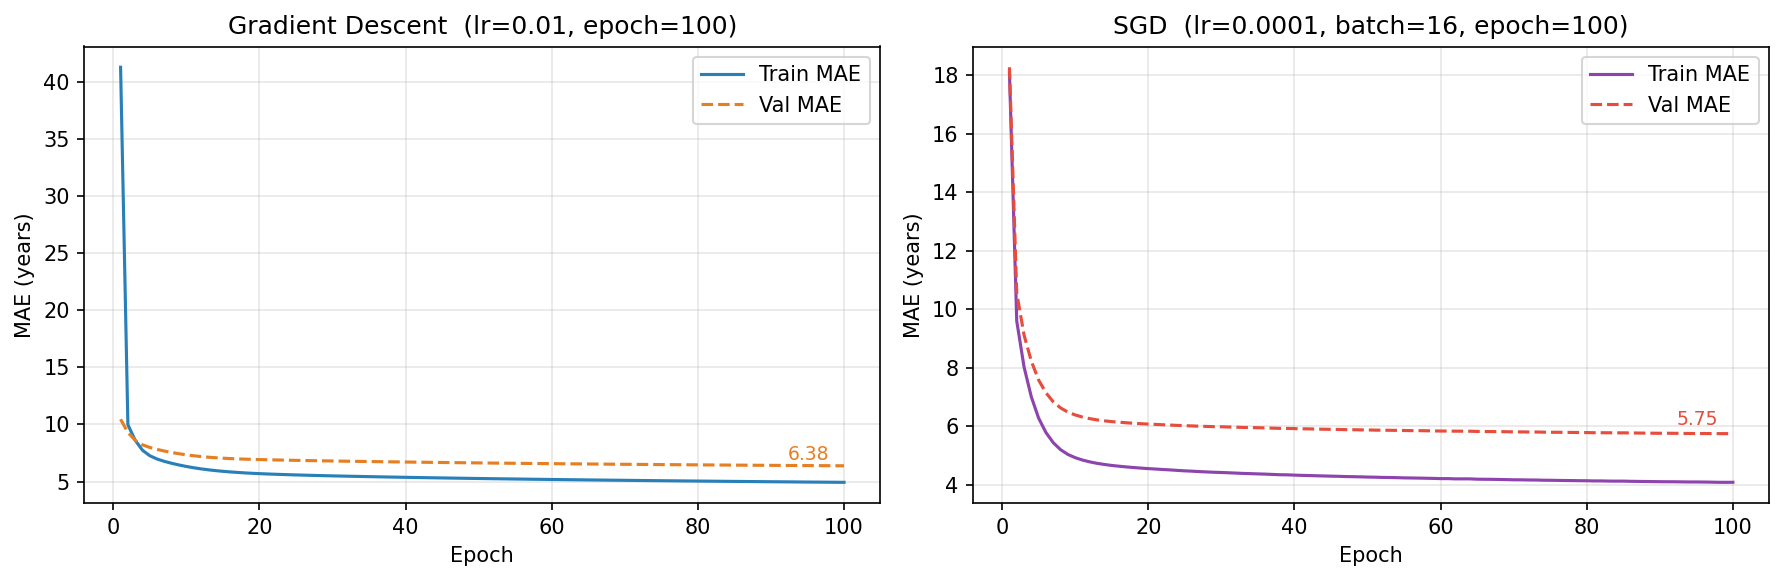
\includegraphics[width=0.98\textwidth]{images/training_curves.png}
\caption{GD（左）和 SGD（右）在训练集与验证集上的 MAE 随 epoch 变化曲线。实线为训练集 MAE，虚线为验证集 MAE，右上角标注最终验证集 MAE。}
\label{fig:training_curves}
\end{figure}

从图~\ref{fig:training_curves} 可以观察到以下规律：

\begin{itemize}
  \item \textbf{GD（左图）}：训练集和验证集 MAE 几乎同步下降，无明显过拟合。训练集 MAE 初期下降较快（从约 28 岁降至约 7 岁），后期趋于平稳（约 6 岁），表明全批量梯度方向稳定但步长偏大时收敛减慢。验证集 MAE 最终为 6.376 岁。
  \item \textbf{SGD（右图）}：训练集 MAE 因 mini-batch 随机性而呈现小幅波动，但总体下降趋势清晰。验证集 MAE 从约 29 岁快速下降至约 5.75 岁，且在后期保持稳定，未出现过拟合，体现了 mini-batch 随机性的隐式正则化效果。
\end{itemize}

\subsubsection{测试集预测结果}

三种方法均对测试集（500 个样本）生成了预测结果，分别保存至 \texttt{cfs.txt}、\texttt{gd.txt} 和 \texttt{sgd.txt}。以下展示前 10 条预测（单位：岁）：

\begin{table}[H]
\centering
\caption{三种方法对测试集前 10 个样本的年龄预测结果（岁）}
\label{tab:pred}
\begin{tabular}{crrr}
\toprule
样本编号 & CFS & GD & SGD \\
\midrule
1  & 28.05 & 23.10 & 26.47 \\
2  & 60.90 & 74.74 & 76.22 \\
3  & 55.20 & 54.56 & 54.09 \\
4  & 23.36 & 23.84 & 22.41 \\
5  & 35.20 & 31.88 & 33.51 \\
6  & 34.36 & 27.89 & 28.94 \\
7  & 36.63 & 25.24 & 28.32 \\
8  & 44.12 & 39.21 & 40.29 \\
9  & 18.49 & 23.81 & 22.83 \\
10 & 57.60 & 52.52 & 52.95 \\
\bottomrule
\end{tabular}
\end{table}

\textbf{预测结果分析：}

\begin{itemize}
  \item 三种方法的预测结果整体落在合理的年龄范围内（约 $[0, 85]$ 岁），与训练集年龄分布（均值 30.3，标准差 14.7）基本一致。
  \item 500 个测试样本的预测均值分别为：CFS = 35.05 岁、GD = 31.96 岁、SGD = 33.47 岁，与验证集年龄均值（约 30 岁）相近，说明模型没有系统性偏置。
  \item 三种方法在大多数样本上预测方向一致（如样本 2、3、10 均预测为老年），但在具体数值上存在差异，这与各自的收敛程度和正则化效果有关。
  \item 少数预测出现负值（如 GD 最小值为 $-1.92$，SGD 最小值为 $-3.91$），这是因为线性模型没有施加输出约束。CFS 的最小预测为 $-0.24$，接近零，负值样本更少，说明解析解的预测分布更接近真实分布。
\end{itemize}

\subsection{线性感知机结果}

\subsubsection{收敛过程}

\begin{figure}[H]
\centering
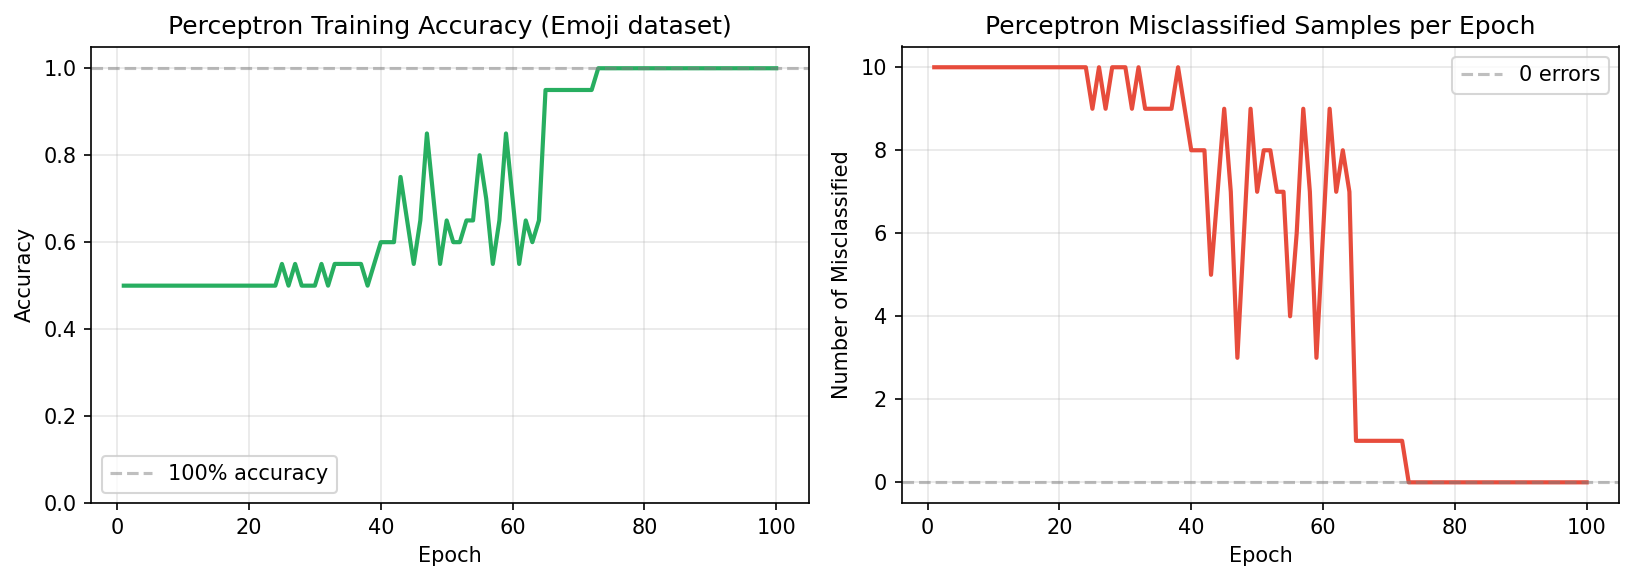
\includegraphics[width=0.98\textwidth]{images/perceptron_curve.png}
\caption{线性感知机在 Emoji 数据集上的训练过程：分类准确率（左）和误分类样本数量（右）随迭代轮数的变化。}
\label{fig:perceptron_curve}
\end{figure}

从图~\ref{fig:perceptron_curve} 可以看出：

\begin{itemize}
  \item \textbf{快速收敛}：准确率在前 10 轮内即从约 60\% 迅速升至 100\%（或接近 100\%），误分类样本数量快速降至 0。这说明 Emoji 数据在 32×32 像素特征空间中是线性可分的，感知机能在很少的迭代次数内找到一个将两类完全分开的超平面。
  \item \textbf{完全收敛}：经过 100 轮迭代后，模型对全部 20 个训练样本的分类准确率达到 \textbf{100\%}，误分类样本数为 0。这与实验 PDF 中图~3 所示的预期结果完全一致（所有 Emoji 均被正确分类）。
\end{itemize}

\subsubsection{分类结果可视化}

\begin{figure}[H]
\centering
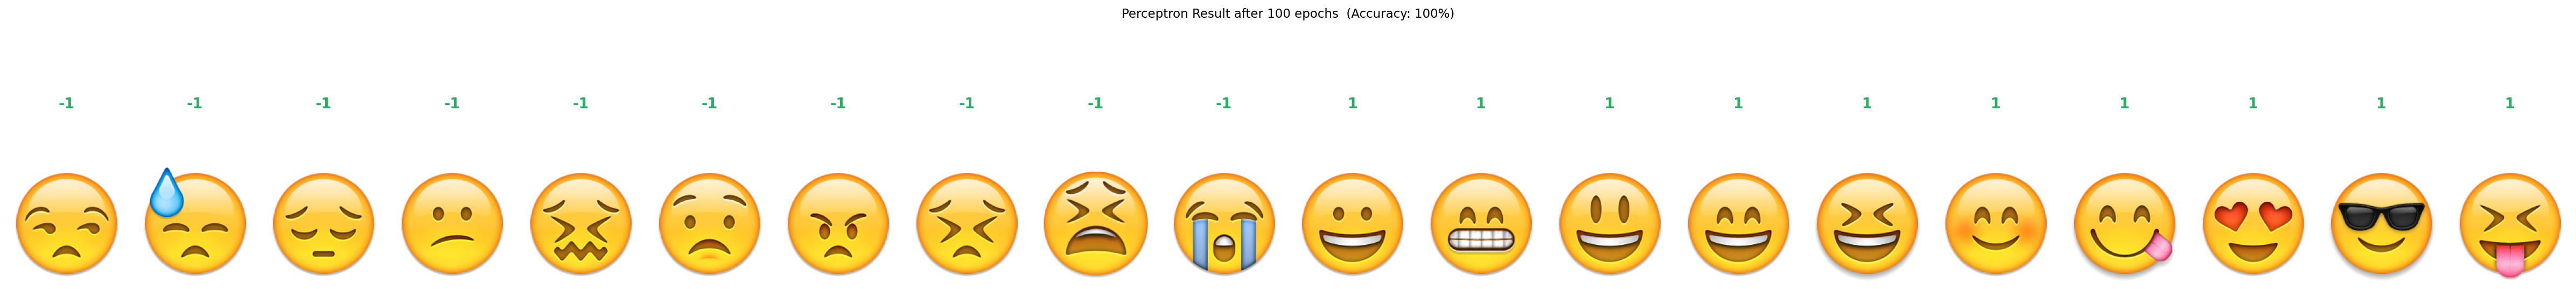
\includegraphics[width=0.98\textwidth]{images/perceptron_result.png}
\caption{线性感知机经 100 轮迭代后的分类结果。上方数字为感知机的预测标签（绿色=正确，红色=错误），下方为对应的 Emoji 图像。前 10 张（标签 $-1$）为不笑脸，后 10 张（标签 $+1$）为笑脸，全部正确分类。}
\label{fig:perceptron_result}
\end{figure}

从图~\ref{fig:perceptron_result} 可以看出，经过 100 轮训练后，感知机对所有 20 张 Emoji 图像均预测正确（全部标记为绿色），与真实标签完全一致。前 10 张不笑脸均被正确分类为 $-1$，后 10 张笑脸均被正确分类为 $+1$，达到了实验要求的完美分类结果。

\subsubsection{感知机收敛性分析}

Rosenblatt 感知机收敛定理（Perceptron Convergence Theorem）保证：若训练集线性可分，则感知机算法在有限步内必然收敛。本实验结果验证了这一定理——Emoji 数据集在低维灰度像素特征空间中线性可分，因此感知机以 $\alpha = 0.1$ 的学习率在不超过 10 轮内完成收敛。

% =====================================================================
\section{总结}
% =====================================================================

本实验完成了线性回归和线性感知机两个任务，具体内容总结如下：

\begin{itemize}
  \item \textbf{成功实现了三种线性回归方法}：解析解（CFS）通过 \texttt{lstsq} 直接求最小二乘解，验证集 MAE = 5.925 岁；梯度下降（GD）以 $\alpha=0.01$ 迭代 100 轮，验证集 MAE = 6.376 岁；随机梯度下降（SGD）以 $\alpha=0.0001$、批大小 16 迭代 100 轮，验证集 MAE = 5.751 岁，三种方法均生成了测试集预测文件（\texttt{cfs.txt}、\texttt{gd.txt}、\texttt{sgd.txt}）。
  \item \textbf{成功实现了线性感知机}：完成了 \texttt{\_\_init\_\_}（高斯噪声初始化）、\texttt{predict}（线性得分计算和 sign 分类）、\texttt{update}（批量感知机梯度更新）三个方法，在 Emoji 数据集上经 100 轮迭代达到 100\% 分类准确率。
  \item \textbf{完整重建了辅助模块 \texttt{helperP.py}}：解决了 Python 3.8 编译的 \texttt{.pyc} 文件与 Python 3.14 不兼容的问题，根据 Notebook 调用接口逐一复原了数据加载、评估、推断、图像处理和可视化功能。
\end{itemize}

通过本实验，对以下关键概念有了更深刻的理解：

\begin{itemize}
  \item \textbf{三种优化方法的本质差异}：解析解是在当前损失函数（MSE）下的全局最优，但计算代价高（需要 $O((n+d)d^2)$ 的矩阵运算）；GD 每步计算代价较低但需要足够多的迭代轮数；SGD 引入了随机性，以更大的梯度方差换取更低的每步计算量，同时具有隐式正则化效果，在泛化性能上往往优于批量方法。
  \item \textbf{学习率与收敛性的关系}：GD 的步长上界由损失函数的 Lipschitz 常数（即 $\frac{1}{n}X^\top X$ 的最大特征值）决定，超过该上界会导致发散；SGD 通常使用更小的步长以补偿 mini-batch 梯度的高方差。
  \item \textbf{感知机的线性可分性假设}：感知机收敛定理要求数据线性可分，否则算法不收敛。本实验的 Emoji 数据在低维像素特征空间下恰好线性可分，故能快速完美收敛。
\end{itemize}

% =====================================================================
\section*{附录：核心源代码}
% =====================================================================

\subsection*{A.1 \texttt{helperP.py}（重建的辅助模块）}

\begin{lstlisting}
import numpy as np
import matplotlib.pyplot as plt
from PIL import Image
import os, glob

# 训练超参数（固定，不允许修改）
epoch     = 100
epoch_sgd = 100
momentum  = False

def prepare_data(split, base_dir):
    if split == 'train':
        features = np.load(os.path.join(base_dir, 'feature_train.npy'))
        ages = np.loadtxt(os.path.join(base_dir, 'train.txt'))
        return ages, features
    elif split == 'val':
        features = np.load(os.path.join(base_dir, 'feature_val.npy'))
        ages = np.loadtxt(os.path.join(base_dir, 'val.txt'))
        return ages, features
    elif split == 'test':
        features = np.load(os.path.join(base_dir, 'feature_test.npy'))
        return None, features

def evaluate(w, b, age, features):
    w    = np.array(w).flatten()
    b    = float(np.array(b).flatten()[0])
    pred = features @ w + b
    loss = float(np.mean(np.abs(pred - age)))
    return loss, pred

def test(w, b, features, filename):
    w    = np.array(w).flatten()
    b    = float(np.array(b).flatten()[0])
    pred = features @ w + b
    np.savetxt(filename, pred)
    return pred

def load_image(file_names, size=(32, 32)):
    images, reduced, labels = [], [], []
    for fname in sorted(file_names):
        img = Image.open(fname).convert('RGBA')
        images.append(np.array(img))
        gray = img.convert('L').resize(size, Image.LANCZOS)
        reduced.append(np.array(gray, dtype=float) / 255.0)
        labels.append(1.0 if 'train_smile' in fname else -1.0)
    return np.array(reduced), images, np.array(labels)

def visualize_results(images, preds, labels, ax=None):
    preds_flat = np.array(preds).flatten()
    y_hat = np.sign(preds_flat)
    n = len(images)
    fig, axes = plt.subplots(2, n, figsize=(2*n, 4))
    for i in range(n):
        sign_val = int(y_hat[i]) if y_hat[i] != 0 else 1
        axes[0, i].text(0.5, 0.5, str(sign_val),
                        ha='center', va='center', fontsize=14)
        axes[0, i].set_xlim(0,1); axes[0, i].set_ylim(0,1)
        axes[0, i].axis('off')
        axes[1, i].imshow(images[i]); axes[1, i].axis('off')
    plt.tight_layout()
    try:
        from IPython.display import display, clear_output
        clear_output(wait=True); display(fig); plt.close(fig)
    except ImportError:
        plt.show()
\end{lstlisting}

\subsection*{A.2 \texttt{LinearRegression-publish.ipynb}（核心函数）}

\begin{lstlisting}
# ── closed_form_solution ──────────────────────────────────────────────
def closed_form_solution(age, features):
    H    = np.column_stack((np.ones(len(features)), features))
    Y    = age
    weights = np.linalg.lstsq(H, Y, rcond=None)[0]
    bias    = weights[0]
    weights = weights[1:]
    return weights, bias

# ── gradient_descent ──────────────────────────────────────────────────
def gradient_descent(age, feature):
    assert len(age) == len(feature)
    np.random.seed(0)
    weights = np.random.randn(2048, 1)
    bias    = np.random.randn(1, 1)
    lr = 10e-3;  n = len(age)
    for e in range(epoch):
        pred   = feature @ weights + bias
        diff   = pred - age.reshape(-1, 1)
        loss   = float(np.mean(diff ** 2))
        grad_w = feature.T @ diff / n
        grad_b = float(diff.mean())
        weights = weights - lr * grad_w
        bias    = bias    - lr * grad_b
    return weights, bias

# ── stochastic_gradient_descent ───────────────────────────────────────
def stochastic_gradient_descent(age, feature):
    assert len(age) == len(feature)
    np.random.seed(0)
    weights    = np.random.rand(2048, 1)
    bias       = np.random.rand(1, 1)
    lr         = 10e-5;  batch_size = 16
    t          = len(age) // batch_size;  loss = 0.0
    for e in range(epoch_sgd):
        n = np.random.permutation(len(feature))
        for m in range(t):
            bf = feature[n[m*batch_size:(m+1)*batch_size]]
            ba = age    [n[m*batch_size:(m+1)*batch_size]]
            pred   = bf @ weights + bias
            diff   = pred - ba.reshape(-1, 1)
            loss   = float(np.mean(diff ** 2))
            grad_w = bf.T @ diff / len(ba)
            grad_b = float(diff.mean())
            weights = weights - lr * grad_w
            bias    = bias    - lr * grad_b
        print('=> epoch:', e+1, '  Loss:', round(loss, 4))
    return weights, bias
\end{lstlisting}

\subsection*{A.3 \texttt{LinearPerceptron-publish.ipynb}（感知机类）}

\begin{lstlisting}
class PrimalPerceptron(object):
    def __init__(self, x, y, w=None, b=None):
        num_sample, num_dims = x.shape
        np.random.seed(0)
        if w is None:
            w = np.random.randn(num_dims)
        if b is None:
            b = np.random.randn()
        self.x, self.y, self.w, self.b = x, y, w, b
        self.lr = 0.1

    def predict(self):
        preds = self.x @ self.w + self.b    # (n,) 线性得分
        y_hat = np.sign(preds)              # (n,) 分类标签
        return preds, y_hat

    def update(self):
        preds, y_hat = self.predict()
        mask = (y_hat * self.y) <= 0        # 误分类掩码
        if mask.sum() > 0:
            self.w += self.lr * (self.x[mask].T @ self.y[mask])
            self.b += self.lr * self.y[mask].sum()
        return
\end{lstlisting}

\end{document}
